\documentclass[10pt,letterpaper]{article}
\usepackage[margin=0.75in]{geometry}
\usepackage{amsmath,amssymb,bm,array,booktabs,tabularx}
\usepackage[shortlabels]{enumitem}
\usepackage[dvipsnames]{xcolor}
\usepackage{fancyhdr}
\usepackage{comment}
\usepackage{tikz}
\setlength{\parindent}{0pt}
\setlength{\parskip}{0.35em}
\renewcommand{\arraystretch}{1.15}
\newcolumntype{Y}{>{\raggedright\arraybackslash}X}
\newcommand{\spacefor}[1]{\vspace{#1}}
\newcommand{\blank}{\rule{1.1cm}{0.4pt}}
\pagestyle{fancy}
\fancyhf{}
\lhead{MA371: Project 1: Mathematical Sciences}
\rhead{AY27-1}
\cfoot{\thepage}
\setlength{\headheight}{14pt}

\begin{document}
\begin{center}
{\Large\bfseries Finding a Defensible Split in a Collaboration Graph}\\
{\large Guided inquiry packet: Mathematical Sciences}
\end{center}
\textbf{Name:} \rule{2.4in}{0.4pt}\hfill
\textbf{Inquiry partners:} \rule{2.25in}{0.4pt}

\textbf{Decision brief.} A program director must place six mathematical-sciences research teams into two seminar cohorts of three. Keeping teams with documented collaborations together may help them exchange ideas, but the administrative draft split was made without examining those ties. Your job is to advise whether to retain that split or recommend another. You must explain what the mathematics establishes, what it does not, and what additional information a decision-maker would need.

\begin{comment}
This is a \emph{static} network question: one graph records observed relationships. There is no time-update rule, fleet, or differential equation. The technical work is to build matrices from the graph, interpret their eigen-information, and test whether a proposed split actually preserves collaborations.
\end{comment}

\textbf{Relevant MA371 connections.} Lesson 17: eigenvalues and eigenvectors. Lesson 18: diagonalization and eigenvector coordinates. You will apply those ideas to a new kind of matrix; adjacency, degree, Laplacian, and graph-cut terminology is introduced here.

\textbf{Suggested class rhythm (50 minutes).} 8 minutes: learn the objects; 12: construct the six-team matrices; 12: interpret the supplied eigen-output; 10: compare splits and challenge the result; 8: outline a defensible memo. The memo and annex are completed individually after class.

\section*{1. Learn the objects with a three-team example}
A \textbf{graph} consists of \emph{vertices} written as singletons $\{i\}$ (here, they represent teams) and \emph{edges} written as pairs $\{i,j\}$ (here, they are documented two-team collaborations). Our edges are undirected: $\{i,j\}=\{j,i\}$. A simple graph has no self-edges $\{i,i\}$ and at most one edge per pair. We initially record whether an edge exists between two vertices, not its strength or quality.

Consider the small path with vertices $1,2,3$ and edges $\{1,2\}$ and $\{2,3\}$:
\[
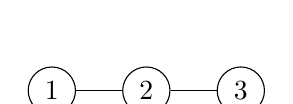
\begin{tikzpicture}[baseline=-0.5ex,every node/.style={circle,draw,minimum size=6mm,inner sep=0pt}]
\node (a) at (0,0) {1}; \node (b) at (1.2,0) {2}; \node (c) at (2.4,0) {3};
\draw (a)--(b)--(c);
\end{tikzpicture}
\qquad
A_{\rm ex}=\begin{bmatrix}0&1&0\\1&0&1\\0&1&0\end{bmatrix},\quad
D_{\rm ex}=\begin{bmatrix}1&0&0\\0&2&0\\0&0&1\end{bmatrix},\quad
L_{\rm ex}=D_{\rm ex}-A_{\rm ex}=
\begin{bmatrix}1&-1&0\\-1&2&-1\\0&-1&1\end{bmatrix}.
\]
The \textbf{adjacency matrix} $A=(A_{ij})$ has entries $A_{ij}=1$ when $\{i,j\}$ is an edge and $0$ otherwise. The \textbf{degree} $d_i$ is the number of neighbors of vertex $i$; the \textbf{degree matrix} $D$ puts those degrees on its diagonal. Note diagonal matrices can be written shortly by specifying only their diagonal entries $D=\text{diag}(1,2,1)$. The \textbf{(combinatorial) Laplacian} is $L=D-A$. Thus $L_{ii}=d_i$ and, for $i\ne j$, $L_{ij}=-1$ for an edge and $0$ otherwise.

\begin{enumerate}[a.,leftmargin=*]
\item Why is $A_{\rm ex}$ symmetric? Why are its diagonal entries zero?\\[0.34in]
\item Verify the second row of $L_{\rm ex}$ from the graph, without subtracting the printed matrices.\\[0.38in]
\item Compute $L_{\rm ex}\vec{1}$ for $\vec{1}=[1,1,1]^T$. Explain in words why every Laplacian built this way satisfies $L\vec{1}=\vec{0}$.\\[0.43in]
\end{enumerate}

\newpage
\section*{2. Build the mathematical model from the case}
The following \emph{synthetic} record documents eight collaborations among six teams. Vertex labels are identifiers, not scores or rankings.
\[
E=\bigl\{\{1,2\},\{1,3\},\{2,3\},\{4,5\},\{4,6\},\{5,6\},\{2,5\},\{3,4\}\bigr\}.
\]
The office's draft assignment is $\{1,2,5\}\mid\{3,4,6\}$. Both cohorts must have exactly three teams. An edge means at least one documented joint problem-solving instance; it does \emph{not} measure how productive the collaboration was. No personnel, scheduling, or security constraints are encoded.

\begin{enumerate}[a.,leftmargin=*]
\item Draw all six labeled vertices and all eight edges. Mark the office's draft split with a line or two colors.\\[1.20in]
\item Build $A$ in the fixed vertex order $1,2,3,4,5,6$. Fill every entry; verify symmetry and the zero diagonal.
\[
A=\begin{bmatrix}
0&\blank&\blank&\blank&\blank&\blank\\
\blank&0&\blank&\blank&\blank&\blank\\
\blank&\blank&0&\blank&\blank&\blank\\
\blank&\blank&\blank&0&\blank&\blank\\
\blank&\blank&\blank&\blank&0&\blank\\
\blank&\blank&\blank&\blank&\blank&0
\end{bmatrix}.
\]
\item Give the degree vector $\vec d=[d_1,\ldots,d_6]^T$ and $D=\operatorname{diag}(d_1,\ldots,d_6)$. What does $\sum_i d_i$ count? Why is it twice the number of edges?\\[0.45in]
\item Construct $L=D-A$. Work out its first and fourth rows explicitly. State the rule you used to fill the others. Check $L\vec{1}=\vec{0}$ using row sums.\\[0.85in]
\item For any vector $\vec z\in\mathbb R^6$, the $i$th entry of $L\vec z$ equals $d_i z_i-\sum_{j\sim i}z_j=\sum_{j\sim i}(z_i-z_j)$. Explain what $j\sim i$ means, then compute $(L\vec z)_2$ in terms of $z_1,\ldots,z_6$.\\[0.5in]
\end{enumerate}

\newpage
\section*{3. Connect the graph to eigenvalues and diagonalization}
 For the three-team path, the following are eigenpairs of its Laplacian:
\[
\begin{array}{c|c}
\lambda&\text{one eigenvector }\vec v\\\hline
0&[1,1,1]^T\\
1&[1,0,-1]^T\\
3&[1,-2,1]^T
\end{array}
\qquad L_{\rm ex}\vec v=\lambda\vec v.
\]
For example, $L_{\rm ex}[1,0,-1]^T=[1,0,-1]^T$: the pattern is unchanged in direction and scaled by $1$. The three distinct eigenvectors form a basis, so $L_{\rm ex}$ is diagonalizable, namely  $L_{\rm ex}=P\Lambda P^{-1}$ with these vectors as columns of $P$ and $0,1,3$ on the diagonal of $\Lambda$ in the same order. This diagonalization can be used to describe the graph's structure.

\begin{enumerate}[a.,leftmargin=*]
\item Verify the eigenpair with $\lambda=3$ by multiplication. What is special about the constant vector for $\lambda=0$?\\[0.55in]
\end{enumerate}

For the six-team graph, a computation reports the Laplacian eigenvalues, in increasing order, as
\[
0,\;1,\;3,\;3,\;4,\;5.
\]
It also reports $\vec u=[1,1,1,1,1,1]^T$ for $\lambda=0$ and $\vec v=[2,1,1,-1,-1,-2]^T$ for the \emph{smallest positive} eigenvalue $\lambda=1$. You are not expected to solve a degree-six characteristic equation by hand. Your task is to check and interpret the supplied output.

\textbf{New interpretation.} For an undirected graph, $L$ is real and symmetric, so it has a basis of real eigenvectors. A zero eigenvalue occurs once per connected component. When the graph is connected, the eigenvector belonging to the smallest positive eigenvalue often gives a useful \emph{candidate} split: group vertices by the signs of its coordinates. The signs are not team quality scores; multiplying $\vec v$ by any nonzero scalar changes neither the eigenpair relation nor the underlying grouping (a negative scalar merely swaps cohort labels).

\textbf{Why this can work.} The identity $\vec z^TL\vec z=\sum_{\{i,j\}\in E}(z_i-z_j)^2$ measures how much a vector's coordinates differ across edges. Among vectors of a fixed length that are orthogonal to $\vec 1$ (their coordinates sum to zero), the smallest-positive-eigenvalue pattern has the least such variation. Its sign changes may therefore reveal a comparatively sparse boundary. This motivates the sign rule; it does \emph{not} prove that the resulting balanced split is optimal. Check the actual edges.

\begin{enumerate}[b.,leftmargin=*]
\item Verify $L\vec v=1\vec v$ for rows 1 and 4 of your matrix. Explain why checking two rows supports, but does not fully verify, the reported eigenpair.\\[0.63in]
\item What does the single zero eigenvalue say about connectivity? Check that conclusion against your drawing.\\[0.42in]
\item Write the two three-team groups suggested by the signs of $\vec v$. Which coordinates are most strongly separated from zero? What would a coordinate near zero make less clear?\\[0.65in]
\item Explain $L=P\Lambda P^{-1}$ for this six-team graph: what do the columns of $P$ and diagonal entries of $\Lambda$ represent? Why does a repeated eigenvalue of $3$ not, by itself, prevent diagonalization here?\\[0.62in]
\end{enumerate}

\newpage
\section*{4. Define success and test the recommendation}
A \textbf{balanced split} is a partition $S\mid S^c$ with $|S|=|S^c|=3$. Its \textbf{cut count} is
\[
C(S)=\#\bigl\{\{i,j\}\in E: i\in S,\ j\in S^c\bigr\}.
\]
This counts \emph{recorded collaborations separated} by the split. The within-cohort edge count is $8-C(S)$. For this fixed eight-edge graph and equally sized cohorts, fewer cut edges means more recorded ties retained inside cohorts. That is the immediate success metric; it is not a measurement of future research quality or a probability of success.

\textbf{Worked mini-check.} On the three-team path, the split $\{1\}\mid\{2,3\}$ cuts $\{1,2\}$ but keeps $\{2,3\}$ within a group, so $C(\{1\})=1$. The six-team calculation is the same kind of edge-by-edge count.

\begin{enumerate}[a.,leftmargin=*]
\item Before counting, predict whether the office's split or the eigenvector-sign split will cut fewer edges. What feature of your graph informs the prediction?\\[0.42in]
\item Fill the table. List the crossing edges so that another cadet can audit each count. For your own split, maintain the $3$--$3$ balance.
\end{enumerate}
\begin{tabularx}{\linewidth}{@{}p{1.38in}p{1.40in}Yp{0.64in}p{0.64in}@{}}
\toprule
Split & $S\mid S^c$ & Crossing edges & $C(S)$ & $8-C(S)$\\
\midrule
Office draft & $\{1,2,5\}\mid\{3,4,6\}$ & \rule{0pt}{0.62in} & & \\
Eigenvector signs & & \rule{0pt}{0.62in} & & \\
Your alternative & & \rule{0pt}{0.62in} & & \\
\bottomrule
\end{tabularx}

\begin{enumerate}[c.,leftmargin=*]
\item Does the sign split outperform the office draft under the \emph{stated} metric? Does the eigenvector equation alone prove that it is the best possible balanced split? Distinguish a suggested candidate from an independently checked count.\\[0.55in]
\item Someone calls $\bigl(8-C(S)\bigr)/8$ the ``chance of successful collaboration.'' What is wrong with that interpretation? Give a precise label for the fraction instead.\\[0.52in]
\end{enumerate}

\textbf{Mathematical interpretation check.} For the three-team path and $\vec z=[1,0,-1]^T$, compute the two squared edge differences and $\vec z^TL_{\rm ex}\vec z$. Explain why they agree.\\[0.34in]

\newpage
\section*{5. Challenge the model, then frame the decision}
\textbf{Data-completeness stress test.} Suppose an audit uncovers two plausible but previously unrecorded collaborations, $\{1,5\}$ and $\{3,6\}$. Consider three scenarios: the original eight-edge record, the record with only $\{1,5\}$ added, and the record with \emph{both} edges added. Do not silently change the original calculation. For this stress test, hold the two \emph{candidate partitions} fixed and recount crossing edges; you do not need to recompute eigenvectors.

\begin{tabularx}{\linewidth}{@{}Yp{1.1in}p{1.1in}Y@{}}
\toprule
Edge record & Office cut & Sign-split cut & What changes in your advice?\\
\midrule
Original eight edges & \rule{0pt}{0.49in} & & \\
Add $\{1,5\}$ only & \rule{0pt}{0.49in} & & \\
Add both edges & \rule{0pt}{0.49in} & & \\
\bottomrule
\end{tabularx}

\begin{enumerate}[a.,leftmargin=*]
\item In the two-edge scenario, is one split still better by cut count? Which original claim becomes less secure?\\[0.52in]
\item Name one other assumption behind treating each edge equally. What real information could reverse a recommendation even if the eight recorded ties are complete?\\[0.55in]
\item The graph is a static snapshot. Explain why the Laplacian eigenvalues here are \emph{not} growth/decay rates or week-by-week forecasts.\\[0.42in]
\end{enumerate}
\newpage
\textbf{AI as a classroom coach (optional).} During the designated class session, an approved AI tool may ask you questions, explain a definition, or critique your reasoning. For example: ``Test whether my crossing-edge list is complete; do not write my recommendation.'' Check its claims against the edge list and your calculations. Do not provide real personnel or sensitive data. Record the tool, your question or purpose, the help received, and how you verified it: \rule{\linewidth}{0.4pt}

\section*{6. Writing your memo}
Before leaving class, record your own provisional decision and its conditions. A defensible decision may be conditional when the evidence is thin.

\begin{tabularx}{\linewidth}{@{}p{2in}Y@{}}
\toprule
Claim & \rule{0pt}{0.43in}\\
\\
\\
\midrule
Mathematical evidence & \rule{0pt}{0.54in}\\
\\
\\
\midrule
Limitation(s) or counterevidence & \rule{0pt}{0.54in}\\
\\
\\
\midrule
Information needed next & \rule{0pt}{0.46in}\\
\\
\\
\bottomrule
\end{tabularx}

\textbf{Final individual product (typed).} Use the instructor's cleaned Army-style executive-summary template. Write a memo of at most two pages to the program director that states your recommendation, the decision criterion, the numerical comparison, and a concrete limitation or condition. Explain the result so a nontechnical leader can use it. Attach a technical annex of at most three pages showing your graph-to-matrix construction, selected eigenpair checks and interpretation, auditable cut counts, and stress-test result. The annex substantiates the memo; the memo should not be a transcript of calculations.

The memo and annex must be your own writing, without AI drafting or rewriting. If you used AI during class, disclose its limited role and your verification. Do not claim that the model proves a personnel outcome or that a small cut count establishes causation.

\end{document}
